\begin{figure}[h!]
    \centering
    \caption{Estimated landlord shares and counterfactual increases in log rents
            and log total wages, Chicago-Naperville-Elgin CBSA}
    \label{fig:map_chicago_cf_rents_wages}

    \begin{minipage}{.95\textwidth} \centering
        (a) Increase in federal MW to \$9
        \vspace{2mm}
    \end{minipage}
    
    \begin{subfigure}{.38\textwidth}
        \caption*{Changes in log rents}
        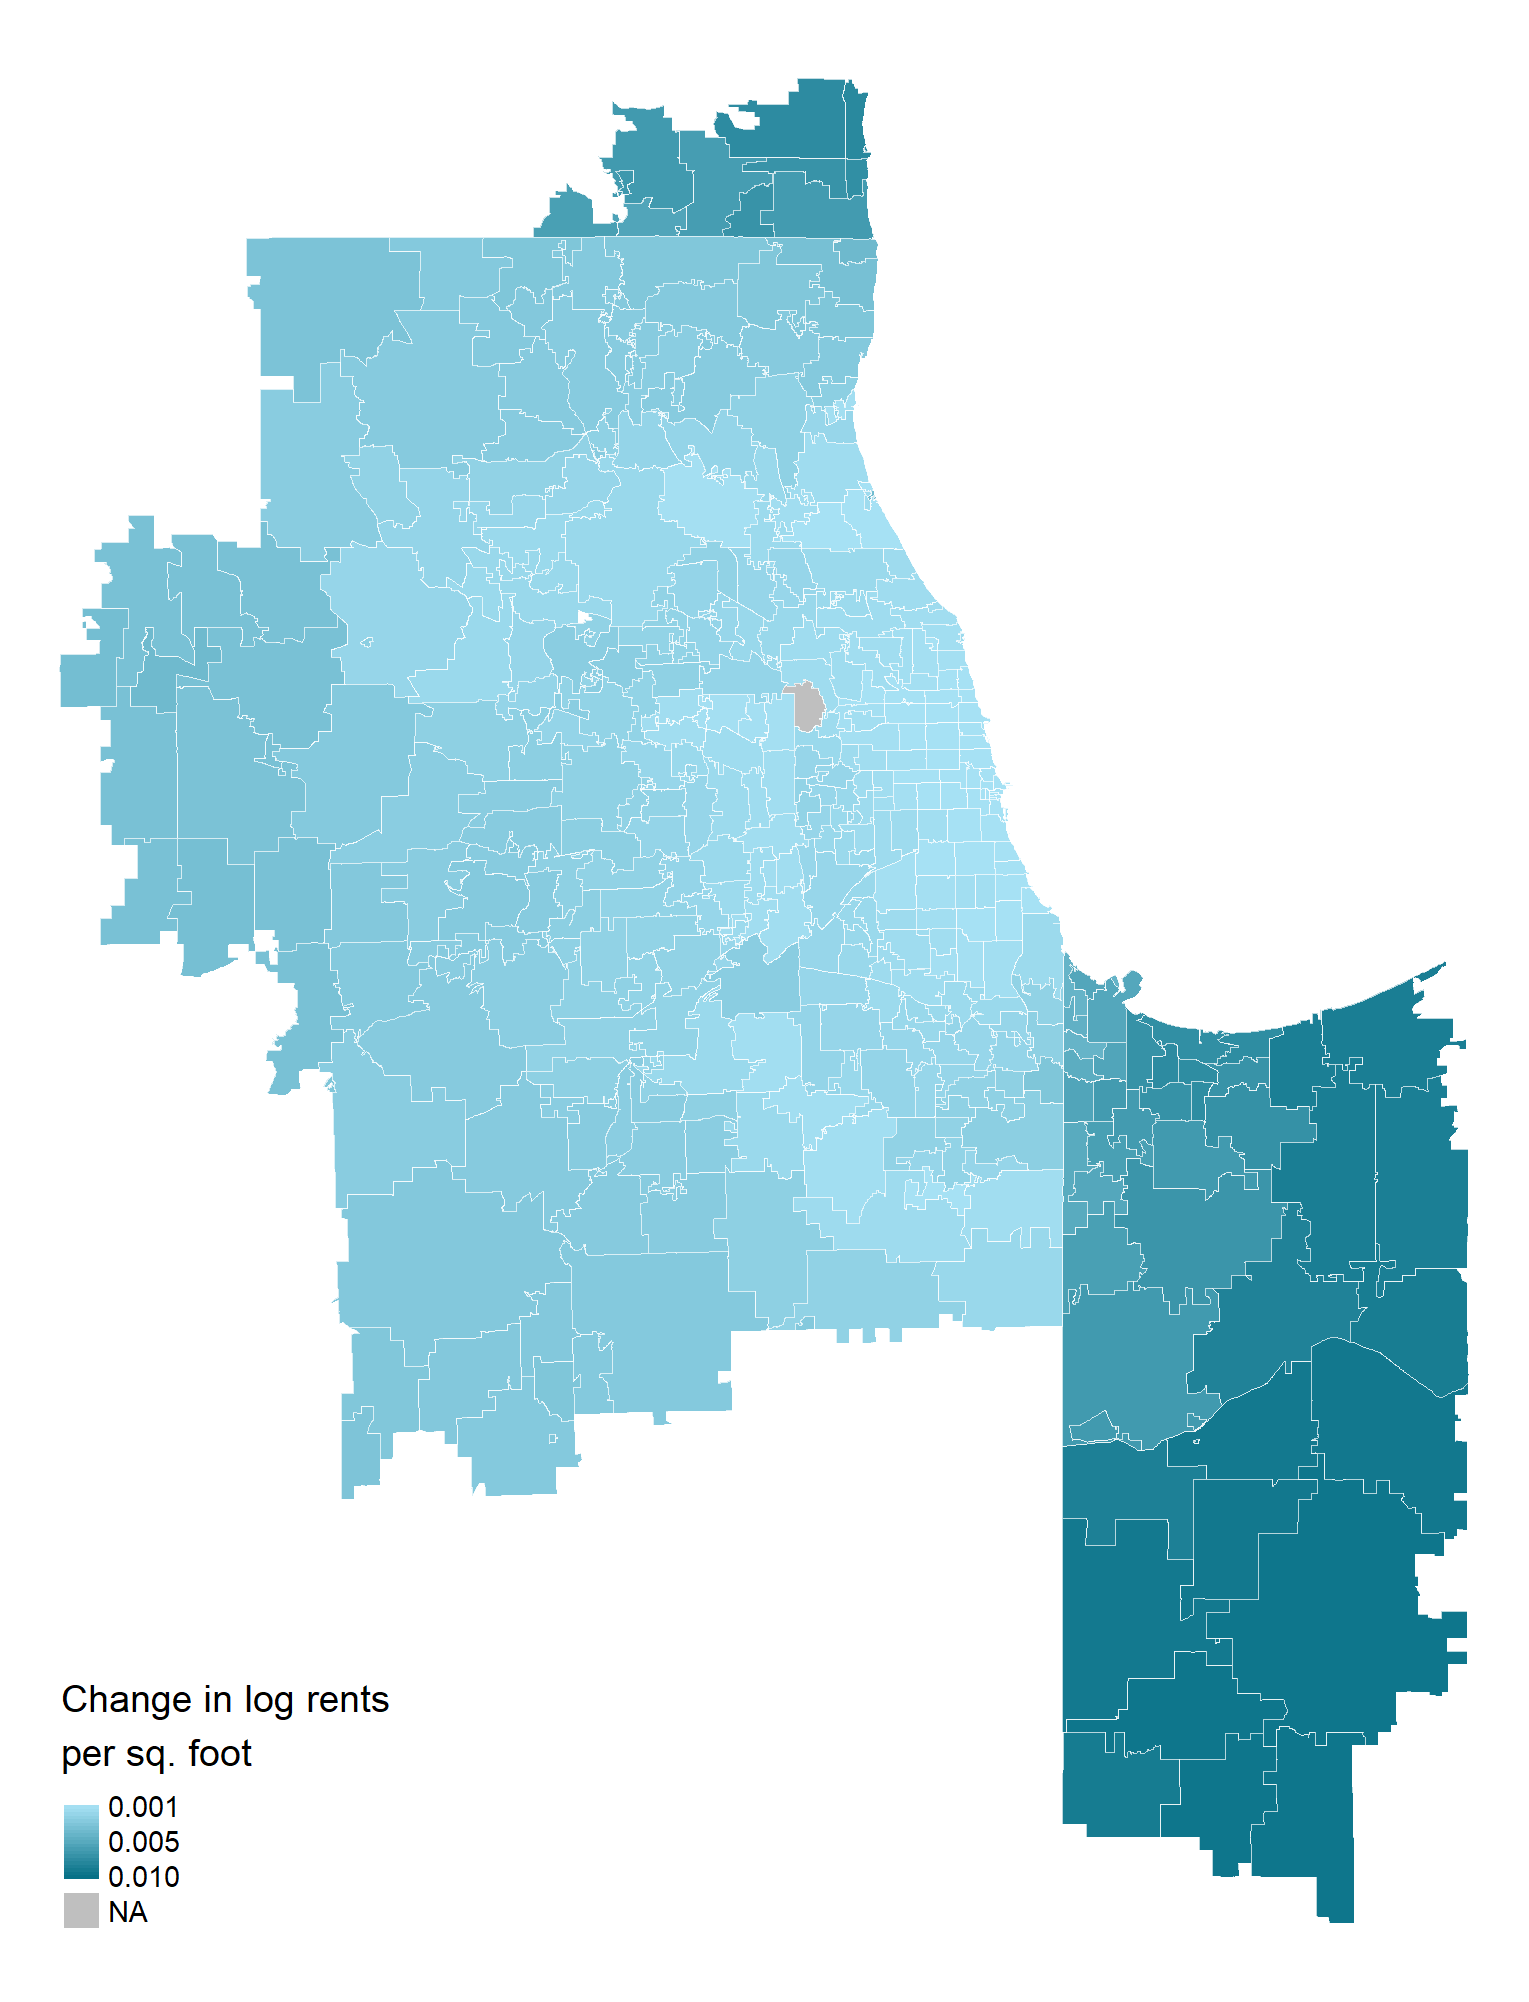
\includegraphics[width = 1\textwidth]
            {counterfactuals/output/chicago_d_ln_rents_fed_9usd.png}
    \end{subfigure}%
    $\quad\quad\quad\quad$%
    \begin{subfigure}{.38\textwidth}
        \caption*{Changes in log total wages}
        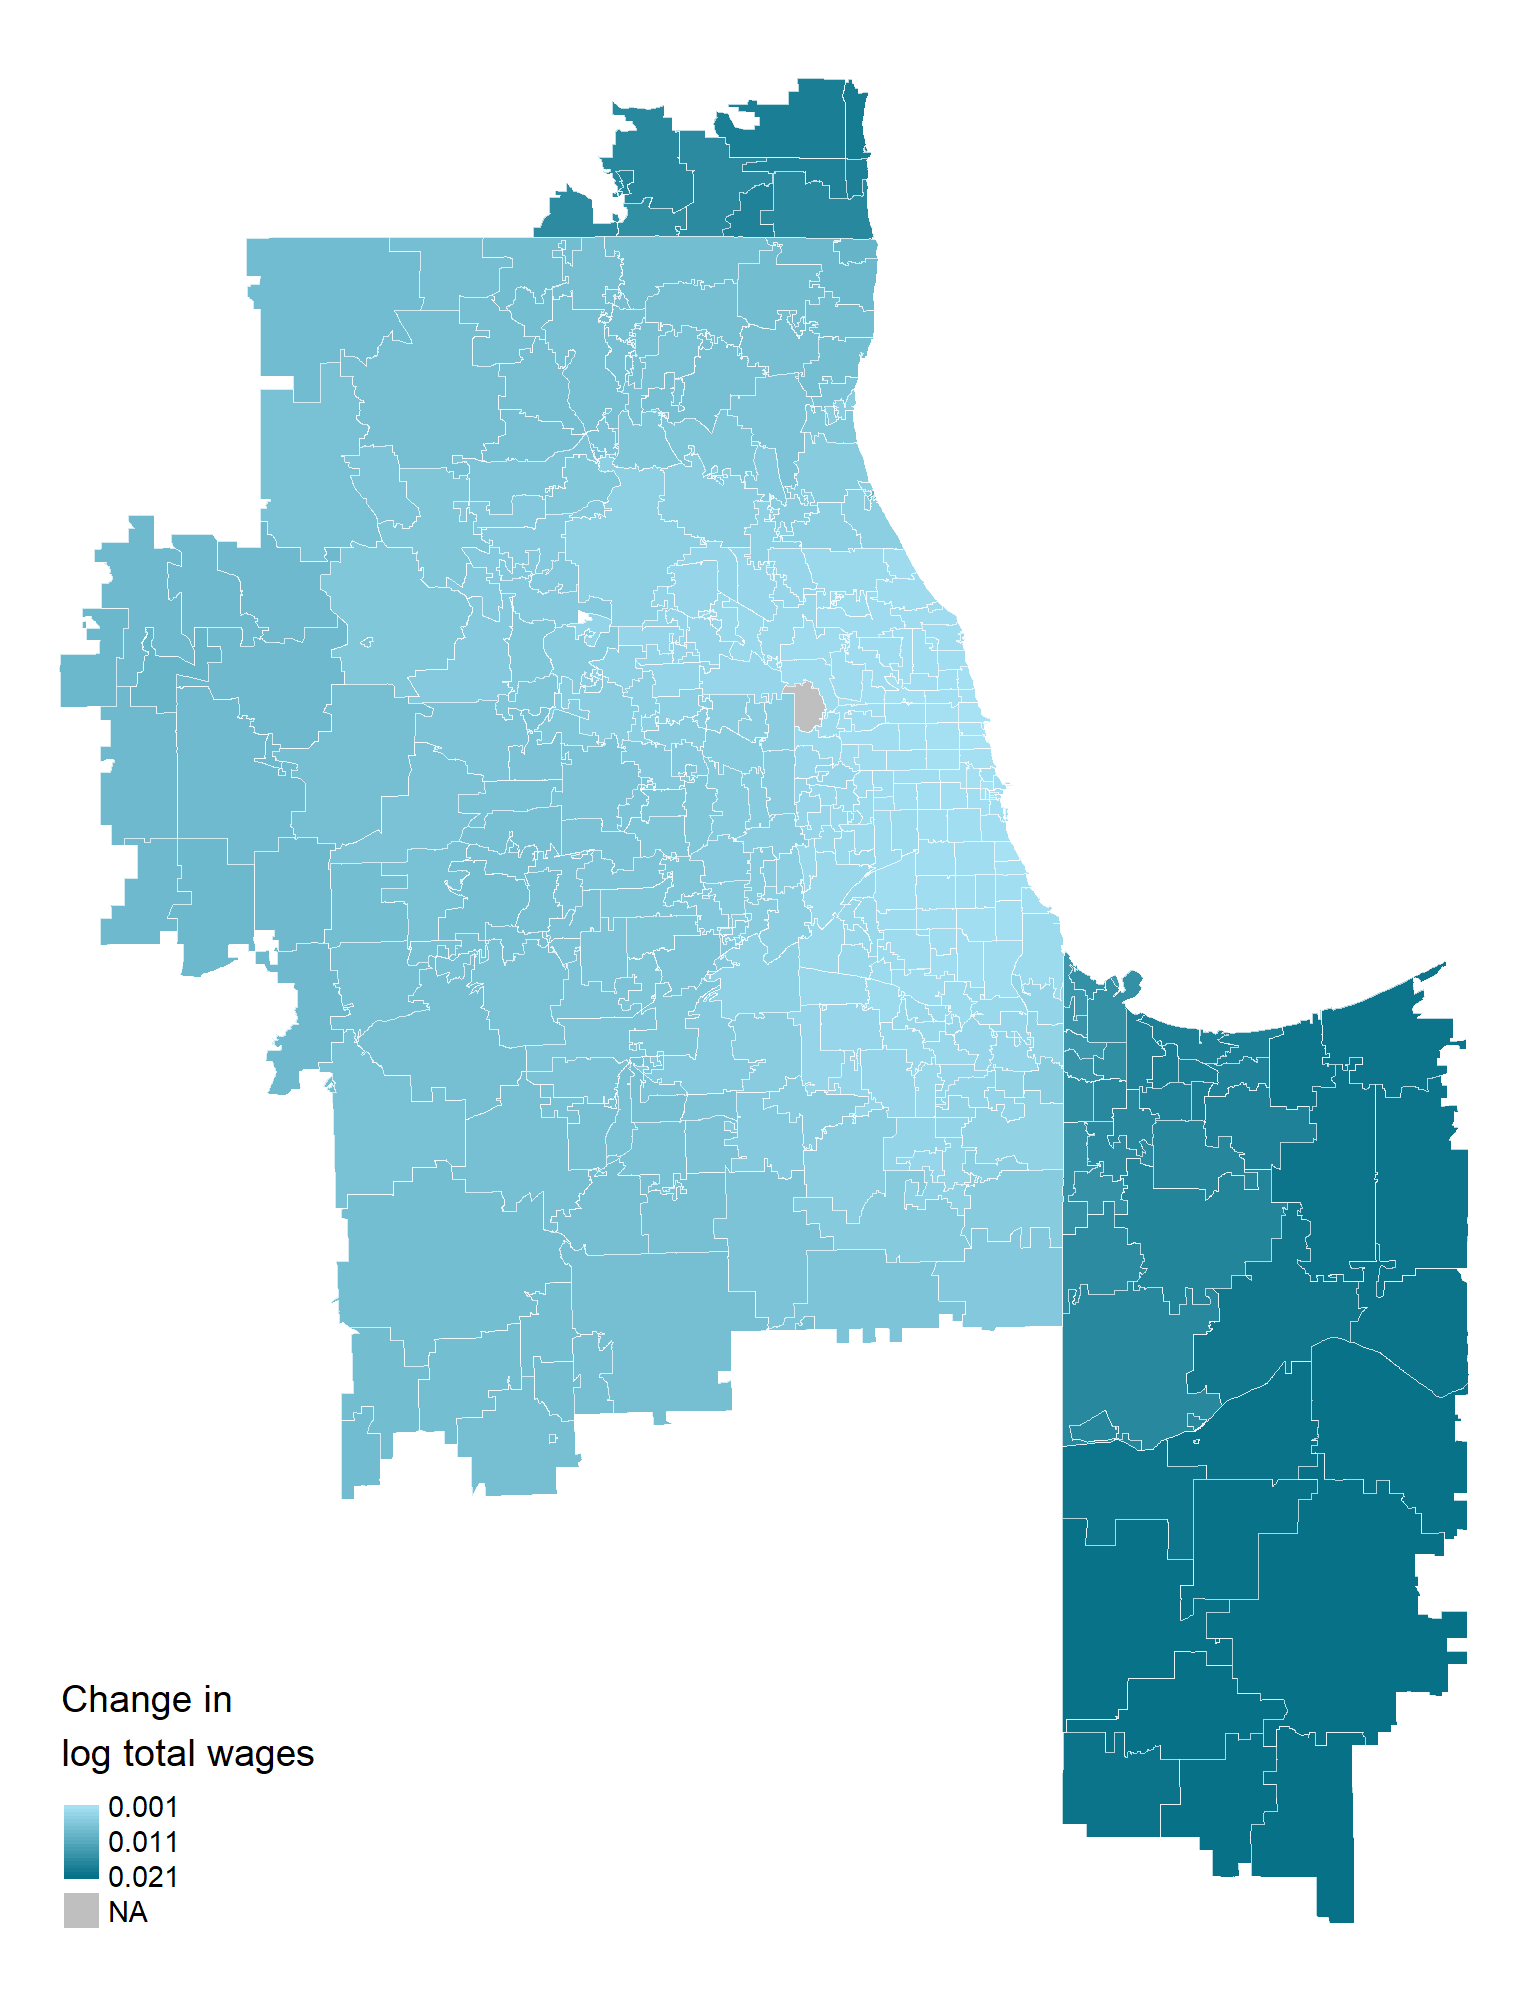
\includegraphics[width = 1\textwidth]
            {counterfactuals/output/chicago_d_ln_wagebill_fed_9usd.png}
    \end{subfigure}

    \begin{minipage}{.95\textwidth} \centering
        \vspace{2mm}
        (b) Increase in Chicago MW to \$14
    \end{minipage}
    
    \vspace{2mm}
    \begin{subfigure}{.38\textwidth}
        \caption*{Changes in log rents}
        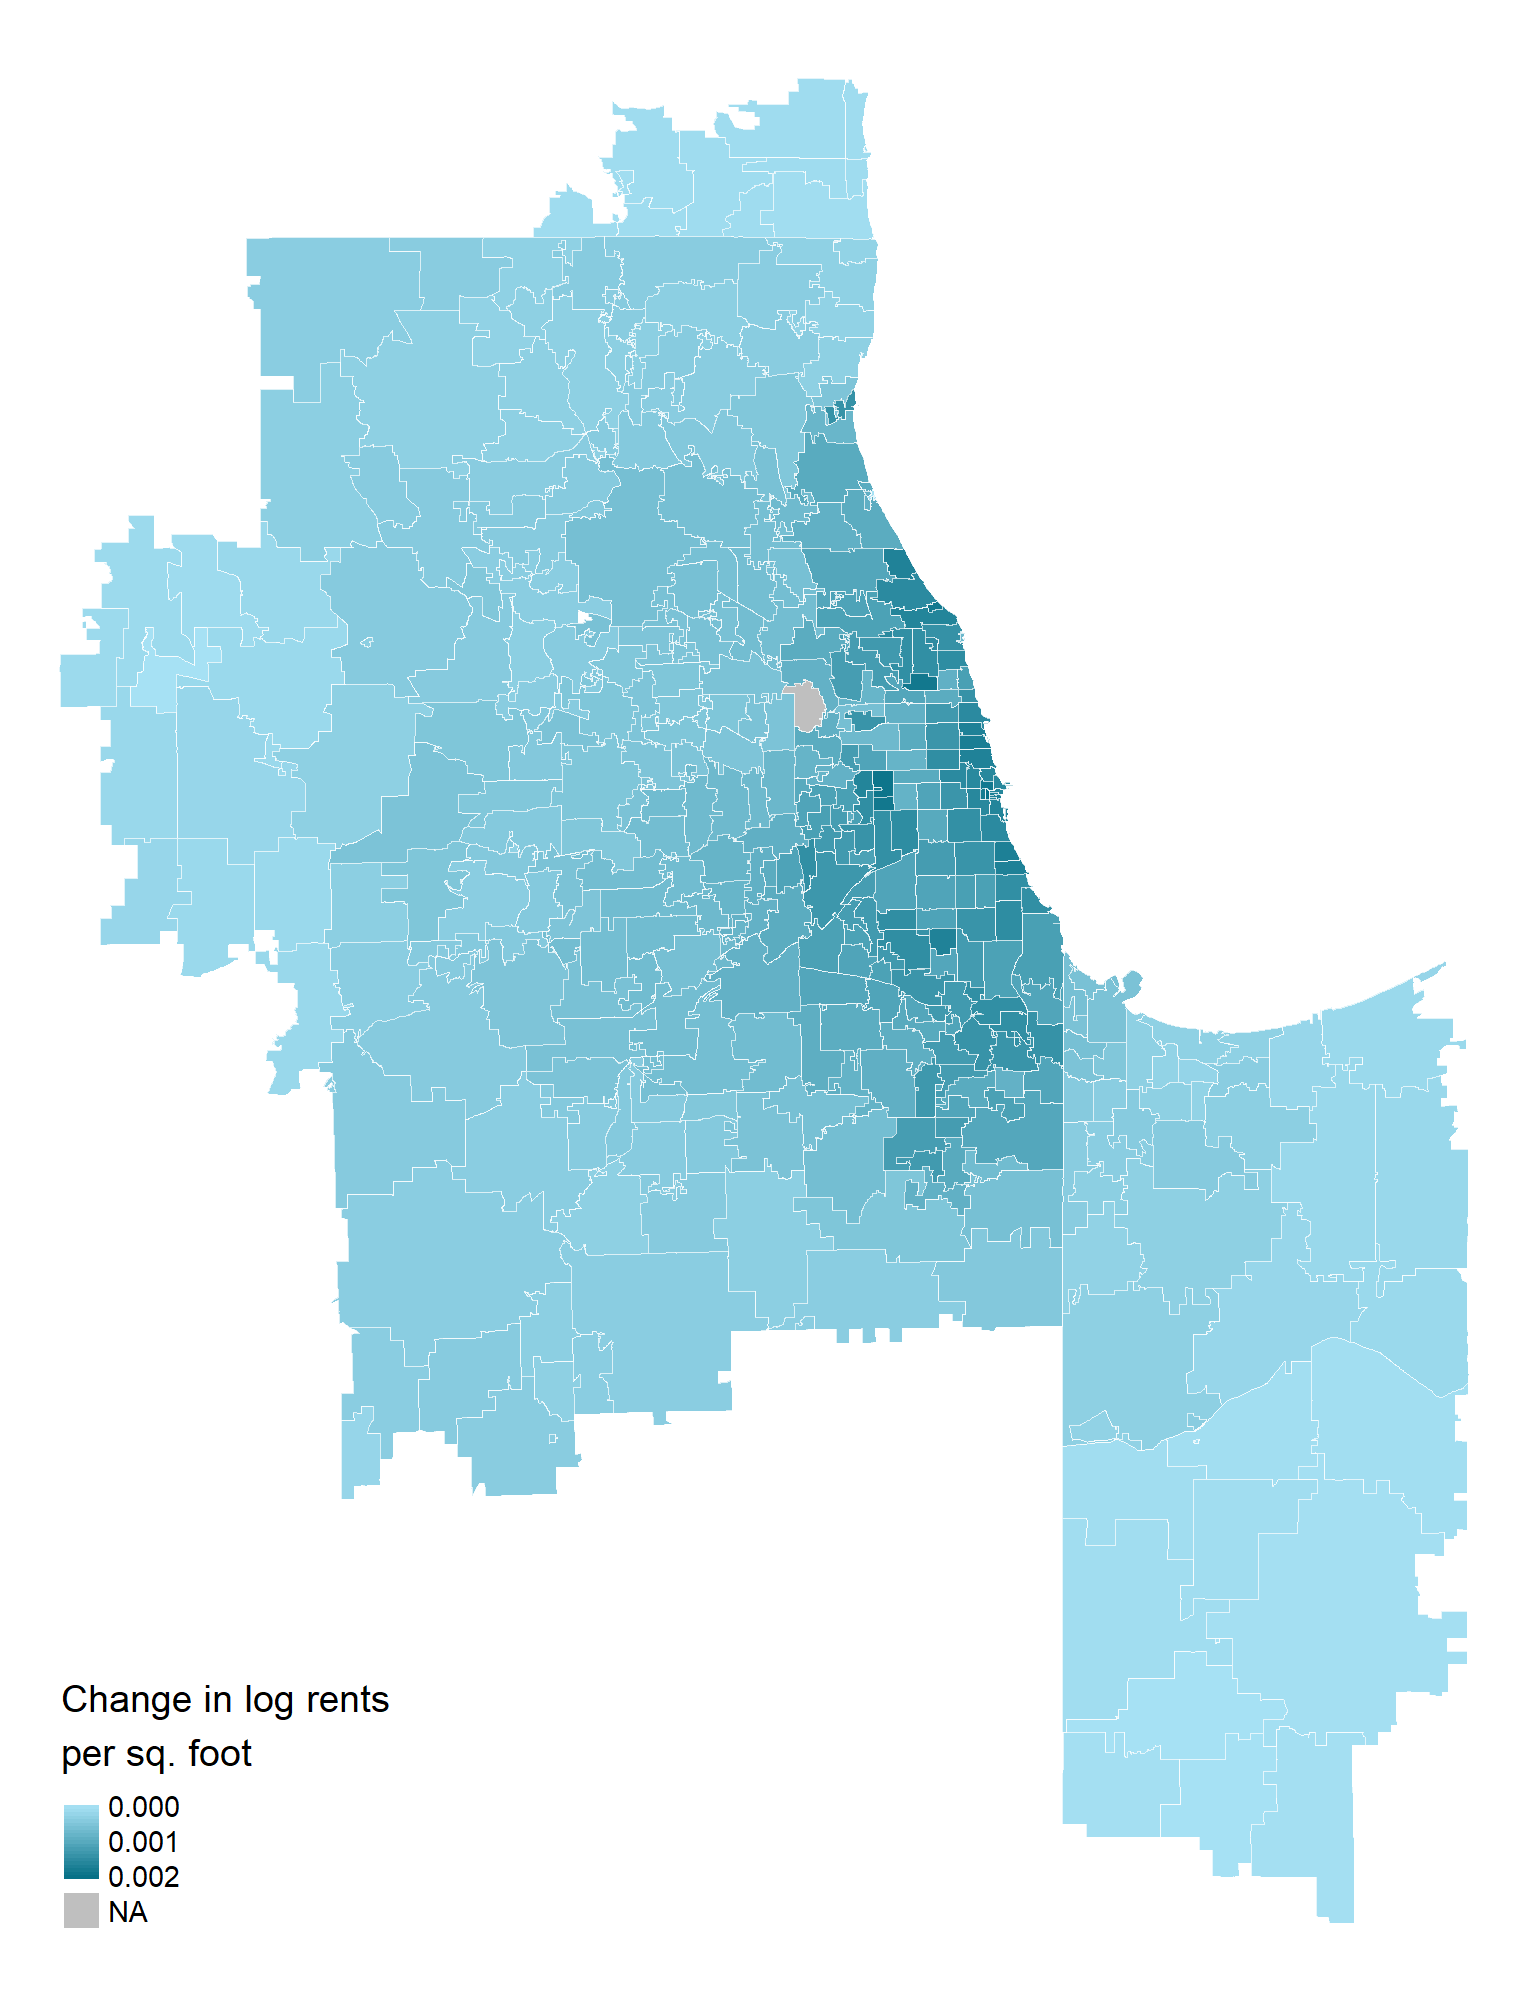
\includegraphics[width = 1\textwidth]
            {counterfactuals/output/chicago_d_ln_rents_chi14.png}
    \end{subfigure}%
    $\quad\quad\quad\quad$%
    \begin{subfigure}{.38\textwidth}
        \caption*{Changes in log total wages}
        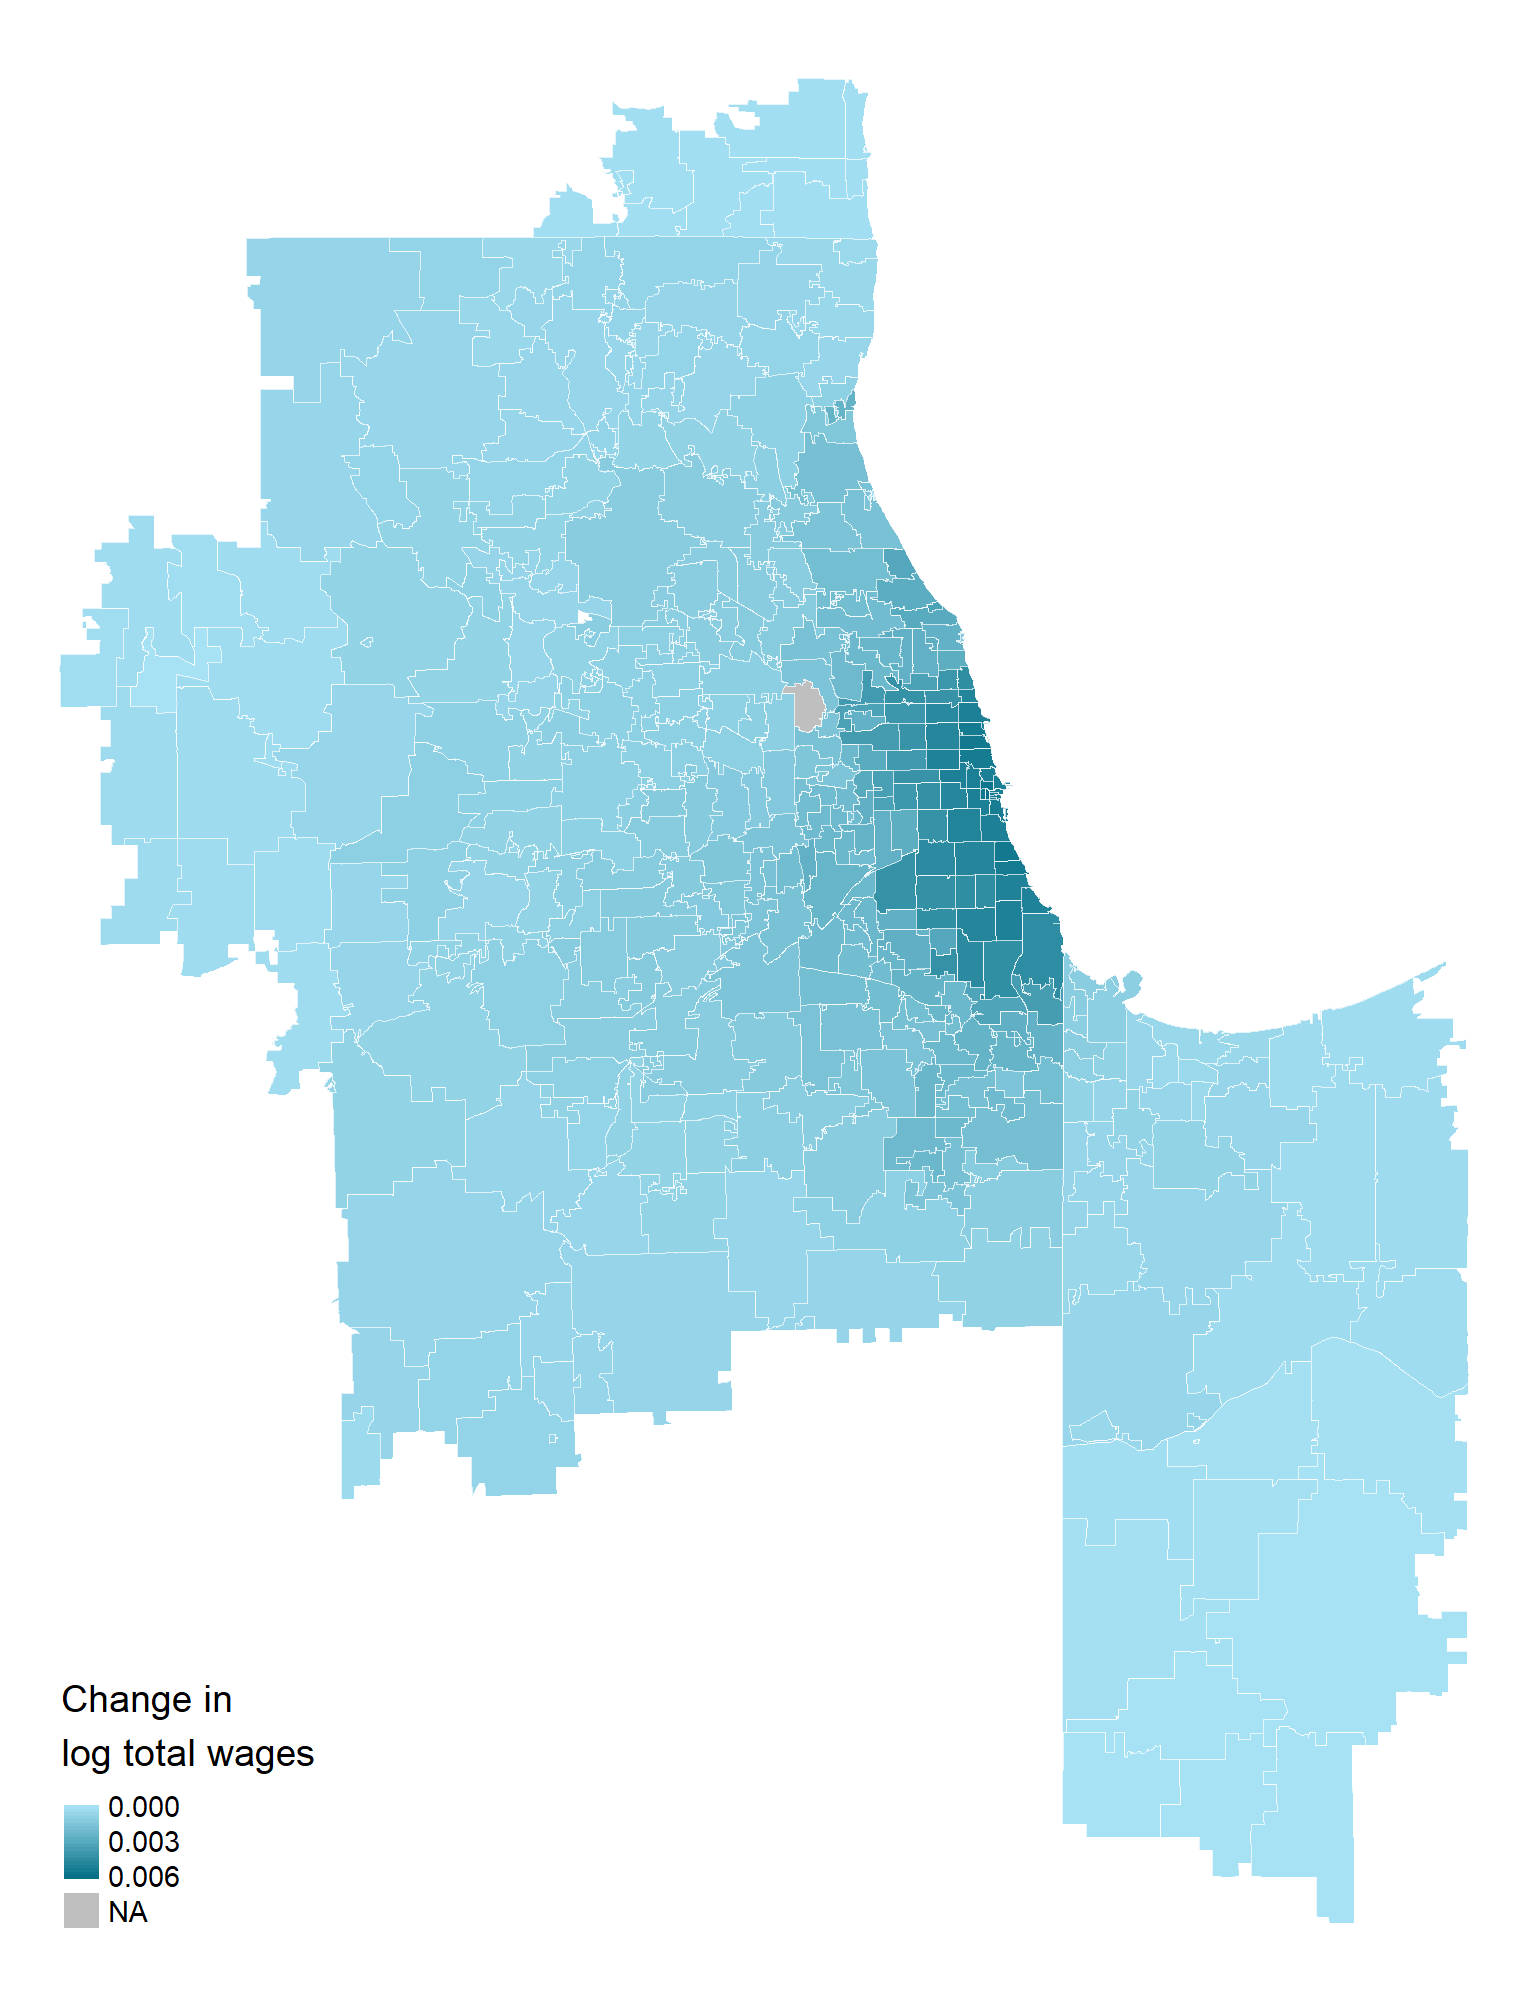
\includegraphics[width = 1\textwidth]
            {counterfactuals/output/chicago_d_ln_wagebill_chi14.png}
    \end{subfigure}

    \begin{minipage}{.95\textwidth} \footnotesize
        \vspace{3mm}
        Notes: 
        Data are from the MW panel described in section \ref{sec:data_mw_panel} 
        and from LODES.
        The figures map the estimated changes in log total rents per square foot
        and log total wage income under different counterfactual MW policies for 
        ZIP codes in the Chicago-Naperville-Elgin CBSA.
        Panel (a) is based on a counterfactual increase to \$9 in the 
        federal MW in January 2020, holding constant other MW policies in their 
        December 2019 levels.
        Panel (b) is based on a counterfactual increase from \$13 to \$14 in the 
        Chicago City MW, also holding constant other MW policies.
        The share pocketed is defined as the ratio between the percent increase 
        in rents and the percent increase in total wages multiplied by the share 
        of housing expenditure in the ZIP code.
        To estimate it we follow the procedure described in Section 
        \ref{sec:counterfactual}, assuming the following parameter values: 
        $\beta = \betaCf$, $\gamma = \gammaCf$, and $\varepsilon = \epsilonCf$.
    \end{minipage}
\end{figure}
